\centering
\vspace{0.5cm}
\tikzstyle{neuronv}=[circle,minimum size=20pt,inner sep=0pt, thick, fill=orange!30, draw=red!50]
\tikzstyle{neuronh}=[circle,minimum size=20pt,inner sep=0pt, thick, fill=blue!20, draw=blue!60]
\tikzstyle{stateTransition}=[thick]
\tikzstyle{learned}=[text=black]
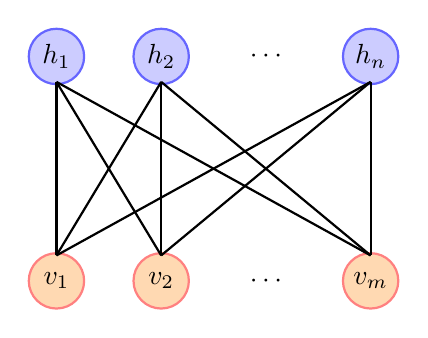
\begin{tikzpicture}[scale=1.9]
    % \draw ;
    \node (v1)[neuronv] at (0, 0) {$v_1$};
    \node (v2)[neuronv] at (0.7, 0) {$v_2$};
    \node (v3)[] at (1.4, 0) {$\cdots$};
    \node (v4)[neuronv] at (2.1, 0) {$v_m$};

    \node (h1)[neuronh] at (0, 1.5) {$h_1$};
    \node (h2)[neuronh] at (0.7, 1.5) {$h_2$};
    \node (h3)[] at (1.4, 1.5) {$\cdots$};
    \node (h4)[neuronh] at (2.1, 1.5) {$h_n$};

	\draw[stateTransition] (0,0.17) -- (0,1.33) node [midway,above=-0.06cm,sloped] {};
    \draw[stateTransition] (0,0.17) -- (0.7,1.33) node [midway,above=-0.06cm,sloped] {};
    \draw[stateTransition] (0,0.17) -- (2.1,1.33) node [midway,above=-0.06cm,sloped] {};

    \draw[stateTransition] (0.7,0.17) -- (0,1.33) node [midway,above=-0.06cm,sloped] {};
    \draw[stateTransition] (0.7,0.17) -- (0.7,1.33) node [midway,above=-0.06cm,sloped] {};
    \draw[stateTransition] (0.7,0.17) -- (2.1,1.33) node [midway,above=-0.06cm,sloped] {};

    \draw[stateTransition] (2.1,0.17) -- (0,1.33) node [midway,above=-0.06cm,sloped] {};
    \draw[stateTransition] (2.1,0.17) -- (0.7,1.33) node [midway,above=-0.06cm,sloped] {};
    \draw[stateTransition] (2.1,0.17) -- (2.1,1.33) node [midway,above=-0.06cm,sloped] {};

\end{tikzpicture}